% BHASHA 2026 (co-located with ICON 2026) -- camera-ready version.
\documentclass[11pt]{article}
\usepackage[final]{acl}

\usepackage{times}
\usepackage{latexsym}
\usepackage[T1]{fontenc}
\usepackage[utf8]{inputenc}
\usepackage{microtype}
\usepackage{inconsolata}
\usepackage{graphicx}
\usepackage{booktabs}
\usepackage{amsmath}
\usepackage{multirow}
\usepackage{array}
% [H] placement, used for the appendix tables/figures so that supplementary
% material sits where it is written instead of drifting onto float-only pages.
\usepackage{float}
\usepackage{needspace}

% Let a large full-width float share a page with text rather than taking one of
% its own (affects the confusion-matrix grid in the appendix).
\renewcommand{\dbltopfraction}{0.92}
\renewcommand{\dblfloatpagefraction}{0.85}
\renewcommand{\textfraction}{0.06}
\renewcommand{\bottomfraction}{0.75}

% acl.sty loads hyperref itself, so PDF metadata must be set afterwards.
\hypersetup{
  pdfauthor={Mrigank Singh},
  pdftitle={Two Failure Profiles in Zero-Shot Cross-Lingual Transfer of a Small Language Model},
  pdfsubject={},
  pdfcreator={},
  pdfproducer={},
  pdfkeywords={}
}

\Urlmuskip=0mu plus 1mu
\makeatletter
\g@addto@macro{\UrlBreaks}{\do\-\do\.}
\makeatother

\title{Two Failure Profiles in Zero-Shot Cross-Lingual Transfer\\
of a Small Language Model}

\author{Mrigank Singh \\
  UPES Dehradun \\
  \texttt{mriganksingh005@gmail.com}}

\begin{document}
\maketitle

% Columns here vary a lot in how much material they carry. Under the default
% \flushbottom LaTeX forces equal column height by stretching the glue around
% section headings, which opens visible gaps mid-column. Let the slack sit at the
% foot of the column instead.
\raggedbottom

\begin{abstract}
Small language models (SLMs) are attractive for offline, private, and
cost-constrained deployment, but supervised data for adapting them is usually
available only in English. We ask what happens to the other languages when a 3B
decoder is fine-tuned on English alone. Fine-tuning Qwen2.5-3B on English tweet
sentiment via QLoRA, we evaluate zero-shot transfer to Spanish, Romanized Hindi,
and Arabic against five reference points, including a fully fine-tuned \mbox{XLM-R}
encoder and two frontier zero-shot models. English-only supervision produces
positive transfer in every target language (\mbox{+0.049} to \mbox{+0.080}
macro-F1 over the untuned base), and on English the 3B model matches or beats both
frontier baselines at 0.058\,s per sample with no API cost. Transfer is not
uniform, however. Using predicted-class rates on balanced test sets as a
diagnostic, we show that English tuning \emph{recalibrates} the model where
transfer succeeds~--- neutral predictions move from 44\% to 32\% on English and
29\% on Spanish, against a 33\% chance rate~--- but leaves it collapsed onto the
neutral class where transfer fails, at 55\% on Hindi and 69\% on Arabic. These two
collapses do not share a single cause. Label probabilities show that on Arabic the
model still separates the classes almost as well as on Spanish: balancing its
decisions, or giving the instruction in Arabic, recovers most of the lost
macro-F1 (0.546 to 0.669 and 0.665). On Romanized Hindi, which the tokenizer
fragments only slightly more than Spanish, class separation itself is weaker,
neither intervention helps much, and the errors are more consistent with a
code-mixed register. A 70B decoder shows neither collapse. The advantage of the
multilingual \mbox{XLM-R} encoder is likewise narrow: \mbox{XLM-R} wins only Arabic, and loses Spanish by 0.101 macro-F1
through the mirror-image pathology of under-predicting neutral at 15\%. We
characterize these as distinct, separately diagnosable failure modes rather than a
single degradation curve.
\end{abstract}

\section{Introduction}
\label{sec:introduction}

Cross-lingual NLP is dominated by two paradigms: heavily pretrained multilingual
encoders \citep{devlin2019bert,conneau2020xlmr} and frontier-scale generative
models \citep{meta2024llama3,geminiteam2025gemini}. Neither fits well where
deployment needs to be offline, privacy-sensitive, or cost-constrained. Generative
small language models (SLMs) do, and parameter-efficient methods
\citep{hu2022lora,dettmers2023qlora} make them practical to adapt on a single
commodity GPU.

That practicality comes with an asymmetry. Labelled task data is abundant in
English and scarce elsewhere, so SLMs are typically tuned on English and then
deployed multilingually. For encoders this recipe is well characterized: transfer
works, and it degrades predictably with typological and script distance
\citep{pires2019multilingual,wu2019beto,karthikeyan2020cross,hu2020xtreme}. For
small generative decoders it is not. Recent small decoders are pretrained on
multilingual data~--- Qwen2.5, which we study, officially supports over 29
languages including Spanish and Arabic \citep{qwen2025modelcard}~--- but their
per-language pretraining mixture is not documented, they are not trained with a
cross-lingual alignment objective, and their transfer behaviour is mediated by a
subword vocabulary, a component known to allocate tokens very unevenly across
languages \citep{rust2021good,petrov2023tokenizers,ahia2023cost}.

This paper asks whether English-only QLoRA tuning of a 3B decoder helps or hurts
the languages it was not tuned on, how that compares to a multilingual encoder
pretrained on 100 languages and to frontier zero-shot models, and whether degraded
transfer is uniform across languages or takes distinct, identifiable forms.

We study these questions on three-class tweet sentiment across English, Spanish,
Romanized Hindi, and Arabic \citep{barbieri2022xlmt}, comparing six configurations
under one shared prompt for every generative model. The goal throughout is
diagnostic: we care about \emph{where} and \emph{how} a monolingually tuned SLM
fails, not about topping a leaderboard.

\paragraph{Contributions.}
\begin{itemize}\itemsep2pt
\item English-only QLoRA tuning yields positive transfer in all four languages,
  and on English the 3B model matches or beats both a 70B and a frontier API model
  while running self-hosted on a single T4 GPU.
\item \textbf{Predicted-class rate on balanced data}~--- a measurement requiring
  no target-language labels~--- separates two failures that macro-F1 conflates:
  English tuning recalibrates the model where transfer succeeds, and leaves it
  collapsed onto the neutral class where it does not.
\item The collapse itself has \textbf{two failure profiles}. On Arabic, the most
  fragmented language in our set, the model still separates the classes, and a
  balanced decision rule or an Arabic instruction recovers most of the gap; on
  Romanized Hindi, fragmented only slightly more than Spanish, class separation
  itself is weaker and neither intervention repairs it. Fragmentation explains
  neither; our error sample suggests code-mixed register drives the Hindi case.
\item The encoder's advantage, meanwhile, is narrow rather than general: \mbox{XLM-R}
  wins only Arabic, and on Spanish fails through the opposite pathology,
  under-predicting neutral at 15\% against a 33\% chance rate.
\end{itemize}

\section{Related Work}
\label{sec:related_work}

\paragraph{Zero-shot cross-lingual transfer.}
Multilingual encoders transfer English supervision to unseen languages by
projecting them into a shared space \citep{devlin2019bert,conneau2020xlmr};
performance falls off for typologically distant and script-divergent targets
\citep{pires2019multilingual,wu2019beto,karthikeyan2020cross,hu2020xtreme}. Joint
multilingual pretraining turns out not to be strictly necessary for this transfer
\citep{artetxe2020cross}, and even nominally monolingual English models see
substantial incidental non-English text during pretraining
\citep{blevins2022contamination}. Adapter- and merging-based methods manipulate
this capacity directly \citep{pfeiffer2020madx,bandarkar2025merging}.

\paragraph{Generative models and monolingual adaptation.}
Generative models transfer instruction-following across languages
\citep{winata2021fewshot,lin2022xglm,muennighoff2023crosslingual,ustun2024aya}.
Closest to our setting, \citet{chirkova2024zeroshot} study zero-shot cross-lingual
transfer in instruction tuning, and \citet{shaham2024pinch} show that even a small
fraction of multilingual tuning data changes multilingual behaviour substantially.
Both examine models considerably larger than 3B and report aggregate quality; we
instead hold the model small, use \emph{zero} multilingual supervision, and focus
on the structure of the resulting errors.

\paragraph{Tokenization as a transfer bottleneck.}
Subword vocabularies \citep{sennrich2016bpe,kudo2018sentencepiece} fragment
under-represented scripts far more aggressively than English, and the
consequences run from quality to cost: tokenizer quality tracks downstream
monolingual performance \citep{rust2021good}, the resulting inequity in sequence
length and inference cost has been quantified directly
\citep{petrov2023tokenizers,ahia2023cost}, and vocabulary allocation has been
linked to multilingual modelling quality more broadly
\citep{limisiewicz2023tokenization}. Recent MRL work continues this line, relating tokenization to
morphology \citep{poelman2025morphology}, vocabulary adaptation
\citep{downey2023embedding}, and script effects in in-context learning
\citep{ma2025transliteration}. We ask whether this literature explains a
concrete, class-level failure, collapse onto a single label, and find that in our
data it does not: the most fragmented language keeps its class information.

\paragraph{Cross-lingual sentiment.}
Tweet sentiment is a standard cross-lingual benchmark
\citep{rosenthal2017semeval,barbieri2020tweeteval}, with known difficulty from
morphologically rich scripts and Romanized code-mixing
\citep{patwa2020semeval}. We use the multilingual tweet sentiment corpus of
\citet{barbieri2022xlmt}.

\section{Experimental Setup}
\label{sec:setup}

\subsection{Data}
We use the \texttt{cardiffnlp/}\allowbreak\texttt{tweet\_sentiment\_}\allowbreak%
\texttt{multilingual} corpus \citep{barbieri2022xlmt}, taking the English,
Spanish, Hindi, and Arabic splits.
Each language provides 1{,}839 training, 324 validation, and 870 test examples.
Test sets are exactly balanced at 290 examples per class, so a single-class
baseline scores 0.1667 macro-F1 and chance-level prediction of any one class is
33.3\%. This balance is what makes the class-level diagnostics in
\S\ref{sec:analysis} interpretable.

One property of this corpus matters for interpretation: the Hindi test split is
100\% Latin script (0 of 870 examples in Devanagari; the training split is 99.9\%
Latin). Hindi transfer here is therefore \emph{intra-script} adaptation to
Romanized, code-mixed text, and Arabic is the only genuine cross-script condition
in our study.

\subsection{Models}
Table~\ref{tab:models} (Appendix~\ref{app:supp}) lists the six configurations. Only English data is ever
used for training. All four generative configurations receive byte-identical
prompts (Appendix~\ref{app:prompt}), so decoder comparisons are not confounded by
prompt engineering. \mbox{XLM-R} is the one architectural contrast we deliberately do not
control: it is a masked-language-model encoder pretrained on 100 languages with
lower-resource languages upsampled \citep{conneau2020xlmr}, whereas Qwen2.5 is a
decoder whose multilingual pretraining mixture is not documented per language,
and that contrast is the point of the comparison. Gemini~2.5~Pro is treated purely as a
frontier API reference, since its parameter count is undisclosed.


\subsection{Training}
QLoRA \citep{dettmers2023qlora} adaptation of \texttt{Qwen2.5-3B-Instruct}
\citep{qwenteam2024qwen25} targets \texttt{q\_proj} and \texttt{v\_proj}
($r{=}16$, $\alpha{=}16$, dropout 0.05) in 4-bit, with effective batch size 16,
learning rate $2{\times}10^{-4}$, cosine schedule, and 0.1 warmup ratio
\citep{han2023unsloth}. \mbox{XLM-R}-base \citep{conneau2020xlmr} is fully fine-tuned
with batch size 32 and learning rate $2{\times}10^{-5}$. Both use early stopping
(patience 2) on validation loss, with the lowest-loss checkpoint retained, and
both are trained under three seeds (42, 123, 456). All training fits a single
16\,GB T4 in roughly three hours total. Per-seed checkpoints are in
Appendix~\ref{app:training}.

\subsection{Evaluation}
Macro-F1 is the primary metric. For the seed-dependent models we report the mean
over three seeds with the sample standard deviation ($n{-}1$ denominator); for
the deterministic
single-run configurations we report 95\% bootstrap confidence intervals over
1{,}000 resamples of the 870 test predictions. The two notations answer different
questions~--- seed variance versus sampling variance~--- and we do not mix them.
Parse failures were zero for all four generative configurations in all four
languages, so no predictions were discarded or substituted and every cell is
scored over the full 870 examples.

\paragraph{Fragmentation.} Tokens per whitespace word is not comparable across
languages: Arabic attaches articles, prepositions and conjunctions to the word, so
its tweets have fewer, longer words. We therefore measure \emph{parity}
\citep{petrov2023tokenizers}: Qwen2.5 tokens in a tweet divided by Qwen2.5 tokens
in its English translation, pooled over each test split. The 2{,}610 non-English
test items were translated with \texttt{gpt-oss-120b} \citep{openai2025gptoss} at
temperature 0, and hashtags, mentions, URLs, punctuation and emoji were removed from
both sides before counting. On 30 items that also have human translations, machine
translation raises parity by 0.03 to 0.10, least for Hindi
(Appendix~\ref{app:parity}), so small differences between languages should not be
over-read. \mbox{XLM-R}, whose vocabulary is of a different type, is not analysed.

\paragraph{Availability.} Training and evaluation code, cached predictions for all
24 model--language cells, the label-probability and target-language-instruction
runs, the error annotations, and the machine translations used for parity are
available at
\url{https://github.com/Mrigank005/slm-cross-lingual-transfer}. The six fine-tuned
checkpoints (three merged QLoRA models and three \mbox{XLM-R} models, one per seed) are on
the Hugging Face Hub under \url{https://huggingface.co/Mrigank005}. The Llama~3.3
70B model we queried (\texttt{llama-3.3-70b-versatile}) has since been withdrawn by
the API provider, so its released cached predictions are the only way to reproduce
that row exactly.

\section{Results}
\label{sec:results}

\begin{table*}[t]
\centering\small
\setlength{\tabcolsep}{5pt}
\begin{tabular}{@{}lcccc@{}}
\toprule
Model & English & Spanish & Hindi (Rom.) & Arabic \\
\midrule
Majority baseline        & 0.1667 [0.154, 0.179] & 0.1667 [0.154, 0.179] & 0.1667 [0.154, 0.179] & 0.1667 [0.154, 0.179] \\
\addlinespace[2pt]
Qwen2.5 3B (zero-shot)   & 0.6752 [0.644, 0.707] & 0.6253 [0.593, 0.657] & 0.4851 [0.450, 0.521] & 0.4880 [0.453, 0.523] \\
Qwen2.5 3B QLoRA (ours)  & \textbf{0.7244} $\pm$ 0.0071 & 0.6759 $\pm$ 0.0169 & 0.5652 $\pm$ 0.0027 & 0.5456 $\pm$ 0.0177 \\
Llama 3.3 70B            & 0.7137 [0.683, 0.741] & 0.6680 [0.637, 0.697] & 0.6484 [0.617, 0.681] & \textbf{0.7334} [0.704, 0.762] \\
Gemini 2.5 Pro           & 0.6950 [0.665, 0.724] & \textbf{0.7313} [0.703, 0.760] & \textbf{0.6798} [0.649, 0.712] & 0.7015 [0.672, 0.732] \\
\mbox{XLM-R}-base (EN FT)       & 0.6710 $\pm$ 0.0050 & 0.5750 $\pm$ 0.0446 & 0.5299 $\pm$ 0.0049 & 0.6147 $\pm$ 0.0192 \\
\bottomrule
\end{tabular}
\caption{Macro-F1 on the 870-example balanced test set of each language.
Seed-dependent rows (QLoRA, \mbox{XLM-R}) give mean $\pm$ sample standard deviation
over seeds 42/123/456; deterministic rows give the point estimate with a 95\%
bootstrap CI (1{,}000 resamples). Best per column in bold.}
\label{tab:main}
\end{table*}

Table~\ref{tab:main} reports all 24 model--language cells; Figure~\ref{fig:bars} in Appendix~\ref{app:supp} plots them.

\paragraph{English-only tuning transfers positively everywhere.}
Relative to the untuned base, QLoRA improves every language: \mbox{+0.0492}
English, \mbox{+0.0506} Spanish, \mbox{+0.0801} Hindi, and \mbox{+0.0576} Arabic.
The largest gain is on Hindi, a language the model was never trained on and whose
Romanized, code-mixed surface form is far from the training register. Task
supervision in one language therefore improves the task behaviour in other
languages too, rather than only fitting English~--- plausibly by drawing on the
multilingual data already seen in pretraining \citep{qwen2025modelcard}.

\paragraph{On the source language, 3B supervision matches scale.}
The QLoRA model reaches 0.7244 on English, above Llama 3.3 70B (0.7137
[0.683, 0.741]) and Gemini 2.5 Pro (0.6950 [0.665, 0.724]). The margin over Llama
is small and its interval overlaps ours, so we read this as parity-or-better
rather than a decisive win; the substantive point is that a 3B model with task
supervision is competitive with a 70B model without it, at a fraction of the cost.
This advantage does not survive the language boundary: averaged over the four
languages, Gemini leads at 0.7019, Llama at 0.6909, and QLoRA at 0.6278.

\paragraph{Scale helps even where script does not change.}
The gap to the frontier models is not confined to Arabic. On Romanized Hindi~---
Latin script, and fragmented by the tokenizer only slightly more than Spanish
(parity 1.26 against 1.22)~--- QLoRA reaches 0.5652 against 0.6484 for Llama and 0.6798 for
Gemini, a shortfall of 0.08 to 0.11 macro-F1 that is larger than the entire
English--Spanish drop. Whatever the frontier models bring to informal, code-mixed
Latin-script text, it is not something 1{,}839 English examples supply. We return
to this in \S\ref{sec:hindi}, where it becomes the key evidence that fragmentation
does not explain the Hindi failure.


\paragraph{The encoder wins exactly one language.}
QLoRA outperforms fully fine-tuned \mbox{XLM-R} on English (+0.0534), Hindi (+0.0353),
and Spanish (+0.1009). \mbox{XLM-R} wins Arabic, 0.6147 versus 0.5456~--- a 12.7\%
relative advantage, under the shared English instruction
(\S\ref{sec:diagnostic} shows that an Arabic instruction changes this). The English-tuned Qwen2.5 3B decoder thus beats the
English-tuned \mbox{XLM-R} encoder on three of four languages, and the encoder's
advantage appears only in the one non-Latin script. Both models are pretrained on
multilingual data, so this is not a contrast between multilingual and monolingual
pretraining; what differs is \mbox{XLM-R}'s 100-language mixture, which upsamples
lower-resource languages, and its architecture. We read the result as an encoder advantage that is specific to
Arabic (or to its script) rather than general, though with four languages we cannot
separate script from language identity.

\paragraph{Efficiency.}
Table~\ref{tab:efficiency} (Appendix~\ref{app:supp}) gives the deployment picture. The QLoRA model labels a
tweet in 0.058\,s on one T4 with no per-call cost; \mbox{XLM-R} is ${\approx}21\times$
faster but gives up 0.101 macro-F1 on Spanish, an accuracy-for-latency trade rather
than a free win. The Llama (0.702\,s) and Gemini (2.751\,s) figures time each
successful API request, so they include the network round trip, provider-side
queuing and, for Gemini, a thinking budget of up to 128 tokens; they are not
directly comparable with the self-hosted figures and indicate only the order of
magnitude.


\section{Analysis}
\label{sec:analysis}

The aggregate scores in \S\ref{sec:results} show degradation but not its shape.
This section argues that the degradation is not one phenomenon but at least two
distinguishable ones, and that class-level prediction rates identify them more
sharply than macro-F1 does.

\subsection{Predicted-class rate as a diagnostic}
\label{sec:diagnostic}

Because every test split is exactly balanced at 290 examples per class, a
calibrated classifier should assign roughly 33.3\% of its predictions to each
label. Deviation from that rate is therefore directly interpretable without
reference to a baseline, and it separates two situations that can produce the same
macro-F1: a model whose errors on a language are spread across all three classes,
and a model that assigns most inputs in that language to a single class regardless
of their content.
Throughout, we say that a model has \emph{collapsed} onto a class in a language
when it assigns that class to far more than the 33.3\% of inputs that belong to
it.
Table~\ref{tab:neutral} reports the share of predictions assigned to neutral for
every model and language.

\begin{table}[t]
\centering\small
\setlength{\tabcolsep}{4pt}
\begin{tabular}{@{}lcccc@{}}
\toprule
Model & EN & ES & HI & AR \\
\midrule
Qwen2.5 3B         & 44.0 & 44.4 & 69.3 & 76.2 \\
Qwen2.5 3B QLoRA   & 32.0 & 29.1 & 55.2 & \textbf{69.3} \\
\mbox{XLM-R}-base         & 24.4 & 14.5 & 37.8 & 38.4 \\
Llama 3.3 70B      & 27.4 & 23.8 & 33.1 & 39.8 \\
Gemini 2.5 Pro     & 41.0 & 32.2 & 42.8 & 52.2 \\
\bottomrule
\end{tabular}
\caption{Percentage of all 870 predictions assigned to the \emph{neutral} class.
Chance is 33.3\% on these balanced splits: values above it indicate
over-prediction of neutral, below it under-prediction. Bold marks the tuned
model's most extreme cell. Seed-dependent rows are means over three seeds.}
\label{tab:neutral}
\end{table}

The table shows what fine-tuning does and does not accomplish. On English the
untuned decoder already over-predicts neutral (44.0\%); QLoRA tuning pulls it to
32.0\%, essentially chance, and the same correction carries over to Spanish
(44.4\% to 29.1\%) without any Spanish supervision. This recalibration is a large
part of what the +0.049 to +0.051 macro-F1 gains on those languages actually
consist of. On Hindi and Arabic the same tuning barely moves the model: 69.3\% to
55.2\% and 76.2\% to 69.3\%, both still far from chance. English supervision thus
corrects the model's over-use of neutral on the languages where its predictions
already follow the input reasonably well, but not on the two languages where most
inputs receive the neutral label whatever their gold class. Predicted labels alone
cannot tell us whether the model still separates the classes on those languages and
is merely biased towards neutral, or has lost that separation.

To separate the two, we re-ran the tuned model and recorded the probability it
assigns to each label word at the first output step (Appendix~\ref{app:c1c2}). On
Arabic the model still ranks the classes almost as well as on Spanish: one-vs-rest
AUC is 0.885 for negative and 0.871 for positive, against 0.899 and 0.901. Adding
one offset per class until the predictions are balanced, which uses the known class
balance but no item labels, raises Arabic macro-F1 from 0.546 to 0.669, close to
Spanish's 0.687. Giving the same instruction in Arabic, with the label words kept in
English, has almost the same effect: macro-F1 0.665 and a neutral share of 26.1\%.
On Hindi the AUCs are lower (0.797 and 0.810), and neither intervention recovers
much (0.599 and 0.577), although the Hindi instruction also lowers the neutral share
to 34.0\%. On Spanish, which does not collapse, the Spanish instruction slightly
lowers macro-F1 (0.659). Both collapses are therefore a bias towards neutral that
depends on the language of the instruction, but only on Hindi does it sit on top of
a genuine loss of class separation.

The frontier and encoder baselines sit in a different regime. Llama 3.3 70B stays
between 23.8\% and 39.8\% everywhere, and \mbox{XLM-R} between 14.5\% and 38.4\%; neither collapses in the
way the 3B decoder does, though both have their own miscalibrations (\mbox{XLM-R}'s
Spanish, \S\ref{sec:xlmr}). We now examine the two collapsed cells in turn, and
argue they arise from different causes.


\subsection{Fine-tuning barely improves neutral}
\label{sec:perclass}

Decomposing the transfer gains by class sharpens the same point.
Table~\ref{tab:delta} (Appendix~\ref{app:supp}) gives the per-class F1 change from base to QLoRA.

English-only supervision improves the positive class by 0.105 on average and the
negative class by 0.057, but the neutral class by 0.016~--- and on Spanish it is
flat at $-0.001$. This holds \emph{on English itself}, where the model has 1{,}839
in-domain labelled examples and neutral still gains only 0.018. Since the collapses in \S\ref{sec:collapse} and
\S\ref{sec:hindi} are precisely over-assignment to neutral, this is consistent with
their persisting after tuning: the gains available from English supervision are
concentrated in the classes that are not failing.

\begin{table}[H]
\centering\small
\setlength{\tabcolsep}{4pt}
\begin{tabular}{@{}lcccc@{}}
\toprule
& \multicolumn{1}{c}{Neutral} & \multicolumn{3}{c}{Recall} \\
\cmidrule(lr){2-2}\cmidrule(lr){3-5}
Model (Arabic) & pred.\ \% & Neg. & Neu. & Pos. \\
\midrule
Qwen2.5 3B        & 76.2 & 0.317 & 0.928 & 0.293 \\
Qwen2.5 3B QLoRA  & 69.3 & 0.363 & 0.902 & 0.407 \\
\mbox{XLM-R}-base        & 38.4 & 0.617 & 0.595 & 0.638 \\
Gemini 2.5 Pro    & 52.2 & 0.683 & 0.855 & 0.555 \\
Llama 3.3 70B     & 39.8 & 0.769 & 0.741 & 0.683 \\
\midrule
\textit{QLoRA, English} & 32.0 & 0.844 & 0.595 & 0.738 \\
\bottomrule
\end{tabular}
\caption{Arabic neutral-class collapse. ``Neutral pred.~\%'' is the share of all
870 predictions assigned to neutral; chance is 33.3\% under the balanced test set.
The final row gives the same model on English for reference. Seed-dependent rows
are means over three seeds.}
\label{tab:collapse}
\end{table}

\subsection{Arabic: a bias, not a loss of signal}
\label{sec:collapse}

Table~\ref{tab:collapse} reports, for each model on Arabic, the neutral prediction
rate alongside the resulting per-class recall.

The base decoder routes 76.2\% of Arabic inputs to neutral, inflating neutral
recall to 0.928 while polar recall falls to 0.317 and 0.293. Its errors are
therefore not spread evenly across classes: most Arabic inputs, whatever their gold
label, are labelled neutral. English-only fine-tuning
\emph{attenuates but does not repair} this: the neutral share moves only to
69.3\%, and while positive recall improves markedly (0.293 to 0.407), negative
recall barely moves (0.317 to 0.363). The same checkpoint on English sits at
32.0\%, so the pathology is specific to Arabic input under an English instruction,
not a property of the model's calibration in general.

The contrast with scale is sharp. Llama 3.3 70B~--- a decoder like Qwen2.5 3B, but
roughly 23 times larger and trained on different data~--- shows no collapse (39.8\% neutral,
recalls 0.769/0.741/0.683) and posts its \emph{highest} single-language score of
all four on Arabic. Gemini sits between the two, over-predicting neutral at 52.2\%
but retaining usable polar recall. Whatever drives the 3B model's collapse is
substantially mitigated at 70B within the same broad architecture, and task
supervision at 3B does not achieve the same.

Arabic is also the most fragmented language in our set: it needs 41\% more
Qwen2.5 tokens than its English translation (parity 1.41), against 26\% for
Romanized Hindi and 22\% for Spanish. Tokens per word would exaggerate this gap,
because Arabic tweets have only 0.71 times as many words as their English
translations, but the difference survives the fairer measure: the 95\% intervals for
Arabic and Hindi do not overlap (Appendix~\ref{app:parity}).
\citet{petrov2023tokenizers} and \citet{ahia2023cost} document this uneven
allocation of vocabulary and measure its cost in sequence length and API price.
Fragmentation does not, however, remove the information the classifier needs: the
label probabilities separate the Arabic classes almost as well as the Spanish ones,
and a balanced decision rule or an Arabic instruction recovers most of the lost
macro-F1 (\S\ref{sec:diagnostic}). Half of our annotated Arabic errors (4 of 8)
show a sentiment-bearing word split across subwords, but three of these four are
classified correctly under the balanced decision rule (\S\ref{sec:qualitative}), so the
split describes what these errors look like rather than what causes them. The
Arabic collapse reflects a strong prior towards neutral when an English instruction
is applied to Arabic text. Script, fragmentation and Arabic's share of pretraining
data are confounded across our four languages, so we cannot say which of them
produces that prior.

\subsection{Hindi: collapse without fragmentation}
\label{sec:hindi}

If subword fragmentation were the whole story, Romanized Hindi should behave like
Spanish. Both are written in Latin script, and their parity is close: Hindi needs
26\% more tokens than its English translation and Spanish 22\%, far below Arabic's
41\%. Hindi does not behave like Spanish. The QLoRA model routes 55.2\% of Hindi inputs to neutral~---
far from the 29.1\% it achieves on Spanish, and much closer to Arabic~--- and
Hindi shows the largest F1 gap from English of any language after Arabic
($-0.159$).

The error analysis points to a different mechanism. Of 46 annotated Hindi errors,
\emph{none} were tokenization artifacts; the most frequent categories were
code-switching or non-standard Romanized spelling (14/46), context-dependent
references (14/46), and ambiguous neutral phrasing (12/46). Romanized Hindi tweets are lexically opaque
to an English-tuned model not because the tokenizer shreds them but because the
orthography is non-standard and the vocabulary is largely unseen: the surface form
is Latin, so the tokenizer produces plausible-looking English-like subwords that
carry no reliable sentiment signal~--- \emph{bhot} (`very') is tokenized as
\emph{b}\,|\,\emph{hot} (Table~\ref{tab:examples}). Fragmentation is moderate, close to
Spanish's, and the semantic content is still unavailable.

This gives two dissociable failure profiles behind the same observable outcome.
Arabic collapses with the highest fragmentation in our set but with its class
information intact, so the collapse is a bias and removing it recovers most of the
gap. Hindi collapses with fragmentation close to Spanish's and with weaker class
separation, which neither a balanced decision rule nor a Hindi instruction repairs.
The parts of this account rest on different evidence, and we want to be explicit
about which is which. That fragmentation cannot explain Hindi is a measurement: its
parity (1.26) is close to Spanish's (1.22), yet it routes 55.2\% of inputs to
neutral where Spanish routes 29.1\%. That the Arabic collapse is a bias over intact
class information is also a measurement (\S\ref{sec:diagnostic}). That register is
the operative cause for Hindi is an inference from 46 annotated errors, and should
be read as the hypothesis our data motivates rather than one it establishes; it
rests on the author's own labels as a native speaker of Romanized, code-mixed Hindi.
Both languages end at the neutral class because neutral is what the model falls
back on: on Hindi when it recovers too little evidence from the input, on Arabic
when the evidence is there but outweighed by a prior towards neutral.

\subsection{The encoder fails through the opposite mechanism}
\label{sec:xlmr}

\mbox{XLM-R}'s most anomalous cell is Spanish (0.5750 $\pm$ 0.0446). It is not the
encoder's lowest macro-F1~--- that is Hindi, at 0.5299~--- but it carries the
study's most extreme single-class dip: neutral-class F1 falls to
0.3614 $\pm$ 0.1065, some 0.32 below the next-weakest class in the same cell, and
that 0.1065 is the largest seed standard deviation we measure anywhere. The mechanism is the mirror image of \S\ref{sec:collapse}: where the
decoder over-predicts neutral on Arabic, \mbox{XLM-R} assigns only 14.5\% $\pm$ 7.9 of
Spanish inputs to neutral, well under the 33.3\% chance rate, and pushes the mass
into the polar classes. Its Spanish negative (0.680) and positive (0.684) F1 are
unremarkable; only neutral fails. The direction is not uniform across languages:
\mbox{XLM-R} sits below chance on English (24.4\%) and Spanish (14.5\%) but slightly
above it on Hindi (37.8\%) and Arabic (38.4\%). Spanish is nonetheless by far the
largest departure from chance in either direction that \mbox{XLM-R} produces, so it is
the extreme of a tendency visible on the source language rather than an isolated
glitch.

That a decoder and an encoder both fail by mis-sizing the same class, in opposite
directions and on different languages, suggests the neutral category is the
fragile one under transfer rather than either architecture being inherently
fragile. Neutral is defined negatively~--- the absence of polarity~--- so it has
no stable lexical signature to transfer, and a model that loses calibration in
either direction hits this class first. We do not have a mechanistic account of
why a generative decoder adapts to Spanish neutrals so much better than a masked
encoder does, and \mbox{XLM-R}'s Spanish macro-F1 itself has a seed standard deviation
of 0.0446,
so part of the 0.101 gap is optimization instability rather than a stable
architectural property. We flag it as an open question rather than a result.

\subsection{Neutral is the hardest class almost everywhere}
Setting aside the majority baseline, which scores zero on two of the three classes
by construction, neutral has the lowest per-class F1 in 16 of the 20 remaining
model--language cells. The four exceptions are exactly the Qwen configurations on
Hindi and Arabic~--- the cells characterized in \S\ref{sec:collapse} and
\S\ref{sec:hindi}. There, neutral stops being the weakest class not because
neutral becomes easier but because the collapse pushes errors outward into the
polar classes, inflating neutral recall at their expense; in three of the four it
becomes the strongest class, and in the fourth (QLoRA on Hindi) it is overtaken
only by positive. The exception is a symptom of the failure mode, not a
counterexample to it.

\subsection{Qualitative error analysis}
\label{sec:qualitative}

We manually annotated randomly sampled QLoRA misclassifications with a
six-category failure taxonomy (Appendix~\ref{app:errors}) and report the items that
at least two of the three seeds misclassify, so that the sample reflects errors of
the model rather than of one seed: 8 Spanish, 8 Arabic and 46 Hindi items (the Hindi
sample was drawn in two rounds). The Hindi items were labelled by the author, a native speaker; the Spanish and Arabic items
were translated and labelled with the help of proficient non-native speakers of
those languages. At this scale it is a hypothesis-generating exercise, and we use it
only to suggest mechanisms that the aggregate metrics cannot distinguish. Representative annotated items, with English glosses and the
tokenization of a key word, are in Appendix~\ref{app:examples}
(Table~\ref{tab:examples}).

The categories separate by language. Arabic errors are led by tokenization
artifacts (4/8), where a sentiment-bearing word is split across subwords and the
prediction falls to neutral. Spanish errors are mostly ambiguous neutral phrasing
(3/8) and cultural idiom (2/8), with a single tokenization case. Hindi errors are
driven by code-switching and non-standard Romanized spelling (14/46) and
context-dependent references to celebrities, politicians and earlier tweets
(14/46), with no tokenization cases at all. The Hindi annotation also surfaced
noise in the benchmark itself: of the 38 items in the second round, 4 are entirely
English, and for 14 the gold label itself is debatable.

The label-probability runs let us check these categories against the model's own
behaviour. Under the Arabic instruction, at least two seeds classify 5 of the 8
Arabic items correctly, and 6 of 8 under the balanced decision rule, including 2 and
3 of the 4 tokenization items; for Hindi the figures are 17 and 12 of 46. Most
annotated Arabic errors are therefore recoverable from the model's own output
distribution and most Hindi errors are not, in line with \S\ref{sec:diagnostic}.

\subsection{Implications}
\label{sec:implications}

Three points follow that we think generalize beyond this corpus.

\paragraph{Aggregate metrics hide the distinction that matters.} Hindi and Arabic
differ by 0.020 macro-F1 for our tuned model~--- a difference no reviewer would
consider meaningful~--- yet Table~\ref{tab:neutral} separates them by 14 points of
neutral-prediction rate, and the label probabilities show that the model keeps its
class information on one and not on the other. A study reporting only macro-F1 would have concluded that the model
degrades similarly on both and reached for a single explanatory mechanism~---
exactly the move our class-level analysis shows would be wrong.

\paragraph{The diagnostic is cheap and prospective.} Predicted-class rate needs
only unlabelled target-language inputs and the knowledge that the deployment
distribution is roughly balanced, not the target-language annotation that is
missing where such models get deployed. A neutral share far from the expected rate warns that the model is
assigning one label to most inputs, and the warning is available before any
labelled evaluation exists.

\paragraph{Remedies should be matched to the failure profile.} On Arabic, where
the class information survives, the fix lies in the decision: in our data a
target-language instruction, or a recalibration that needs only the expected class
balance, recovers most of the gap. Neither helps much on Romanized Hindi, where
fragmentation is already close to Spanish's and the difficulty is lexical and
register-level; there, a small amount of in-language or code-mixed instruction data
is the more plausible intervention \citep{shaham2024pinch}, which we do not test.

\section{Conclusion}
\label{sec:conclusion}

Fine-tuning a 3B generative SLM on English alone transfers positively to every
language we tested, and on the source language it matches or beats models an order
of magnitude larger while running self-hosted on one commodity GPU with no API cost.
But the transfer is
structured, not uniform, and reading it off aggregate macro-F1 obscures the
structure. Predicted-class rates on balanced data show that English supervision
does one specific thing well: it recalibrates a decoder that already
over-predicted neutral, and that correction transfers to Spanish for free. On
Hindi and Arabic the same supervision leaves it defaulting to neutral~--- 55\% of
Hindi inputs and 69\% of Arabic ones.

Those two collapses look identical in the metric and are not the same failure.
On Arabic, the most fragmented language in our set, the model still separates the
classes; the collapse is a prior towards neutral that a balanced decision rule or
an Arabic instruction largely removes. On Romanized Hindi, fragmented only slightly
more than Spanish, class separation itself is weaker, neither intervention repairs
it, and the errors are more consistent with code-mixed register. Fragmentation
explains neither collapse. Neither
the encoder's multilingual pretraining nor task supervision addresses both: \mbox{XLM-R}
wins only Arabic and fails Spanish through the inverse pathology, while the 70B
decoder avoids both collapses without any task supervision at all.

Practically, a QLoRA-adapted SLM is a sound choice for Latin-script targets in a
familiar register; elsewhere, the neutral-prediction rate is a
cheap pre-deployment check~--- it requires only unlabelled inputs and a balanced
reference, and it flags the collapse before any labelled evaluation exists. The
question our design cannot settle is where the Arabic prior towards neutral comes
from: script, fragmentation, or the pretraining scarcity that co-occurs with them.
Separating them requires holding script constant while varying the tokenizer, for
instance by evaluating Devanagari alongside Romanized Hindi.

\section*{Limitations}

Our evidence comes from a single task, a single corpus, and four languages, only
one of which (Arabic) uses a non-Latin script; the Hindi split is entirely
Romanized, so this study contains no Devanagari condition and cannot speak to
cross-script transfer beyond Arabic. Because fragmentation, script, and
pretraining representation are confounded across these four languages, we cannot
say which of them produces the Arabic prior towards neutral. Our parity estimates rest on machine
translation, which on the human-translated subset raised parity by 0.03 to 0.10;
and because Romanized Hindi tweets are partly English, those segments pass through
translation almost unchanged, which pushes Hindi parity towards 1~--- in the
direction that favours our argument, so the Hindi--Spanish comparison should be read
as approximate. With only four languages we do not correlate fragmentation with
macro-F1; such a correlation would not be statistically meaningful. Our test sets, while exactly balanced, are limited to 870 examples
per language, so the class-level rates in \S\ref{sec:analysis} should be read with
that scale in mind. Compute
constraints limited us to three seeds, so our variance estimates are coarse~---
relevant for \mbox{XLM-R}'s Spanish result, where the seed standard deviation is large
enough that we treat part of that gap as optimization instability. The two
frontier baselines were each run once through their APIs and are subject to
sampling non-determinism we did not measure, and Gemini's undisclosed parameter
count makes any efficiency comparison against it approximate. In addition, the error
taxonomy rests on 62 annotated examples (8 Spanish, 46 Hindi, 8 Arabic), each
labelled by a single annotator, so it
carries no inter-annotator agreement estimate and is offered as
hypothesis-generating rather than as measurement; the Spanish and Arabic labels
and glosses were produced with proficient but non-native speakers, so that part of
the evidence is weaker than the Hindi annotation. We intend the scale comparison
to show that the collapse is mitigated at 70B, not to claim that parameter count
is the operative variable; Llama and Qwen differ in pretraining data and tokenizer
as well as size. The main comparison drives every generative model with an
\emph{English} instruction, which holds the prompt constant across systems. Our
target-language results show that this choice matters, as prior work leads one to
expect \citep{etxaniz2024think}, but they rest on one instruction per language,
written by us with the label words kept in English, and only the Qwen models were
re-run with it; other wordings may behave differently, and Llama and Gemini might
gain from it too. The balanced decision rule assumes that the class balance is
known, which holds for our test sets but not in general deployment. Lastly, the
remedy we suggest for Romanized Hindi, in-language or code-mixed instruction data,
is motivated by the analysis but not tested.

\section*{Ethical Considerations}

The corpus we use consists of public tweets distributed by
\citet{barbieri2022xlmt}. We collected no new data, did not attempt to
re-identify any author, and redistribute no text. Pseudonymisation in the released
data is partial rather than complete, which we think is worth stating: most
mentions and links are masked as \texttt{@user}, \texttt{@someUSER} and
\texttt{http}, but across the 3{,}480 test items we evaluate, 72 (2.1\%) still
carry an unmasked handle (75 distinct) and 39 (1.1\%) still carry a live
\texttt{t.co} link. Anyone reusing this benchmark should not treat it as
de-identified.

The failure mode we document has a distributional cost that we want to state
plainly. A model that routes 69\% of Arabic inputs to the neutral class does not
fail uniformly~--- it systematically erases expressed sentiment, and it does so
for the language in our study whose script the tokenizer handles worst. Deploying
an English-tuned SLM as though its English-language accuracy carried over would
therefore under-report both positive and negative opinion for exactly the users
already least well served by the tokenizer. This is our argument for reporting
predicted-class rates rather than aggregate accuracy before deployment: the
aggregate metric conceals the disparity, and the disparity falls on
under-represented languages.

Two further limits on how these results should be read. The gold labels come with
the corpus and we did not re-annotate them; the items are short and stripped of
conversational context, and what counts as \emph{neutral} is not culturally
invariant, so some of what we score as model error may be disagreement about the
label rather than failure to recover it. And our
error taxonomy was annotated by the author (with non-native speakers'
help for the Spanish and Arabic items), who was not blind to the hypothesis under
test, so it is reported as hypothesis-generating rather than as
evidence. We see no dual-use concern specific to this work beyond those already
attaching to sentiment classification generally.

% acl.sty already issues \bibliographystyle{acl_natbib}; repeating it here makes
% BibTeX report "Illegal, another \bibstyle command".
\bibliography{references}

\appendix

% Arabic snippets are pre-rendered with LuaLaTeX (arabic/build.sh) so that the
% paper itself still compiles with pdfLaTeX.
\newcommand{\arsnip}[1]{\raisebox{-0.3\height}{\includegraphics{arabic/#1}}}

\begin{table*}[!t]
\centering\scriptsize
\setlength{\tabcolsep}{3pt}
\renewcommand{\arraystretch}{1.15}
\begin{tabular}{@{}>{\raggedright\arraybackslash}p{0.5cm}>{\raggedright\arraybackslash}p{4.5cm}>{\raggedright\arraybackslash}p{4.2cm}>{\raggedright\arraybackslash}p{1.2cm}>{\raggedright\arraybackslash}p{1.6cm}>{\raggedright\arraybackslash}p{2.8cm}@{}}
\toprule
Lg. & Text (excerpt) & English gloss & Gold\,$\rightarrow$ pred. & Category & Split of key word \\
\midrule
AR & \arsnip{ar32_text.pdf} \,[two heart emoji] & Nawal El Zoghbi, the voice of calmness [two heart emoji] & pos$\rightarrow$neu & tokenization & `calmness': \arsnip{ar32_split.pdf} \\
AR & \arsnip{ar48_text.pdf} & Michel Aoun spends his days on wishful thinking \ldots\ and the garbage is still there & neg$\rightarrow$neu & tokenization & `the garbage': \arsnip{ar48_split.pdf} \\
\midrule
HI & Awesome stay blessd dear ..! nd b aware in delhi bhot khatarnak jagah hai .. & Awesome, stay blessed dear! And be careful, Delhi is a very dangerous place & neu$\rightarrow$pos & code-switching & \emph{bhot} `very': b\,|\,hot; \emph{khatarnak} `dangerous': k\,|\,hat\,|\,arn\,|\,ak \\
HI & ldko me to sb chalta h yr \ldots\ u mst hv cntrl & With boys anything goes, man \ldots\ you must have control & pos$\rightarrow$neu & code-switching & \emph{ldko} `boys': ld\,|\,ko; \emph{cntrl}: cn\,|\,trl \\
HI & bhai apna time barabaad mat karo kisi ko koi rply nai milne wala & Bro, don't waste your time, nobody's going to get a reply & neg$\rightarrow$neu & code-switching & \emph{barabaad} `wasted': bar\,|\,aba\,|\,ad; \emph{rply}: r\,|\,ply \\
HI & Are kaisi hai Tbyat theek nai hai yr & Hey, how's your health? Not well, man? & neg$\rightarrow$neu & code-switching & \emph{Tbyat} `health': T\,|\,by\,|\,at; \emph{theek} `fine': the\,|\,ek \\
\midrule
ES & Si tu día esta amargo ``pues dale una movida'' aveces el azúcar esta en el fondo. & If your day is bitter, ``give it a stir'': sometimes the sugar is at the bottom. & neu$\rightarrow$pos & cultural idiom & --- \\
ES & Me gusta estar sola y me molesta la gente que habla mucho \ldots & I like being alone, and people who talk a lot annoy me \ldots & neu$\rightarrow$neg & ambiguous neutral & --- \\
\bottomrule
\end{tabular}
\caption{Representative QLoRA misclassifications from the annotated sample
(Appendix~\ref{app:errors}); ``pred.'' is the label predicted by the majority of
the three seeds. Texts are excerpts of the original tweets; glosses
are the English translations recorded with the annotations. ``Split'' is the
Qwen2.5 tokenization of the named word as it occurs in the tweet, with pieces
separated by a bar (Arabic read right to left).}
\label{tab:examples}
\end{table*}

\section{Configurations and Supplementary Results}
\label{app:supp}

\begin{table}[H]
\centering\small
\setlength{\tabcolsep}{3.5pt}
\begin{tabular}{@{}llll@{}}
\toprule
Configuration & Type & Params & Training \\
\midrule
Majority baseline    & Trivial & ---  & none \\
Qwen2.5 3B           & Decoder & 3B   & none \\
Qwen2.5 3B QLoRA     & Decoder & 3B   & EN QLoRA \\
Llama 3.3 70B        & Decoder & 70B  & none \\
Gemini 2.5 Pro       & Decoder & n/a  & none \\
\mbox{XLM-R}-base           & Encoder & 278M & EN full FT \\
\bottomrule
\end{tabular}
\caption{Evaluated configurations. All generative models share one prompt; all
training is English-only. The majority baseline assigns the same single class to
every input; because the test splits are exactly balanced, that ``majority'' is a
three-way tie and which class wins is incidental, so its macro-F1 is 0.1667
either way.}
\label{tab:models}
\end{table}

\begin{table}[H]
\centering\small
\setlength{\tabcolsep}{4pt}
\begin{tabular}{@{}lccc@{}}
\toprule
Model & s/sample & Avg.\ F1 & Cost/1K \\
\midrule
\mbox{XLM-R}-base        & 0.0027 & 0.5976 & \$0 \\
Qwen2.5 3B QLoRA  & 0.058  & 0.6278 & \$0 \\
Llama 3.3 70B     & 0.702  & 0.6909 & \$0.03--0.06 \\
Gemini 2.5 Pro    & 2.751  & 0.7019 & variable \\
\bottomrule
\end{tabular}
\caption{Seconds per sample (mean over the four languages) against mean macro-F1.
Self-hosted rows: batch time on one T4 divided by batch size (\mbox{XLM-R} forward pass at
batch size 32; QLoRA generation at batch size 8). API rows (Llama, Gemini):
wall-clock time of each successful request, including network latency, so the two
groups are not directly comparable. Gemini
was run on a free development tier; production pricing is per-token.}
\label{tab:efficiency}
\end{table}

\begin{table}[H]
\centering\small
\setlength{\tabcolsep}{5pt}
\begin{tabular}{@{}lccc@{}}
\toprule
Language & Negative & Neutral & Positive \\
\midrule
English  & $+0.026$ & $+0.018$ & $+0.104$ \\
Spanish  & $+0.092$ & $-0.001$ & $+0.060$ \\
Hindi    & $+0.069$ & $+0.024$ & $+0.147$ \\
Arabic   & $+0.042$ & $+0.022$ & $+0.109$ \\
\midrule
Mean     & $+0.057$ & $+0.016$ & $+0.105$ \\
\bottomrule
\end{tabular}
\caption{Per-class F1 change from the untuned Qwen2.5 3B to the English-tuned
QLoRA model. Gains concentrate in the polar classes; the neutral class is
essentially unmoved in every language, including English.}
\label{tab:delta}
\end{table}

\begin{figure}[H]
\centering
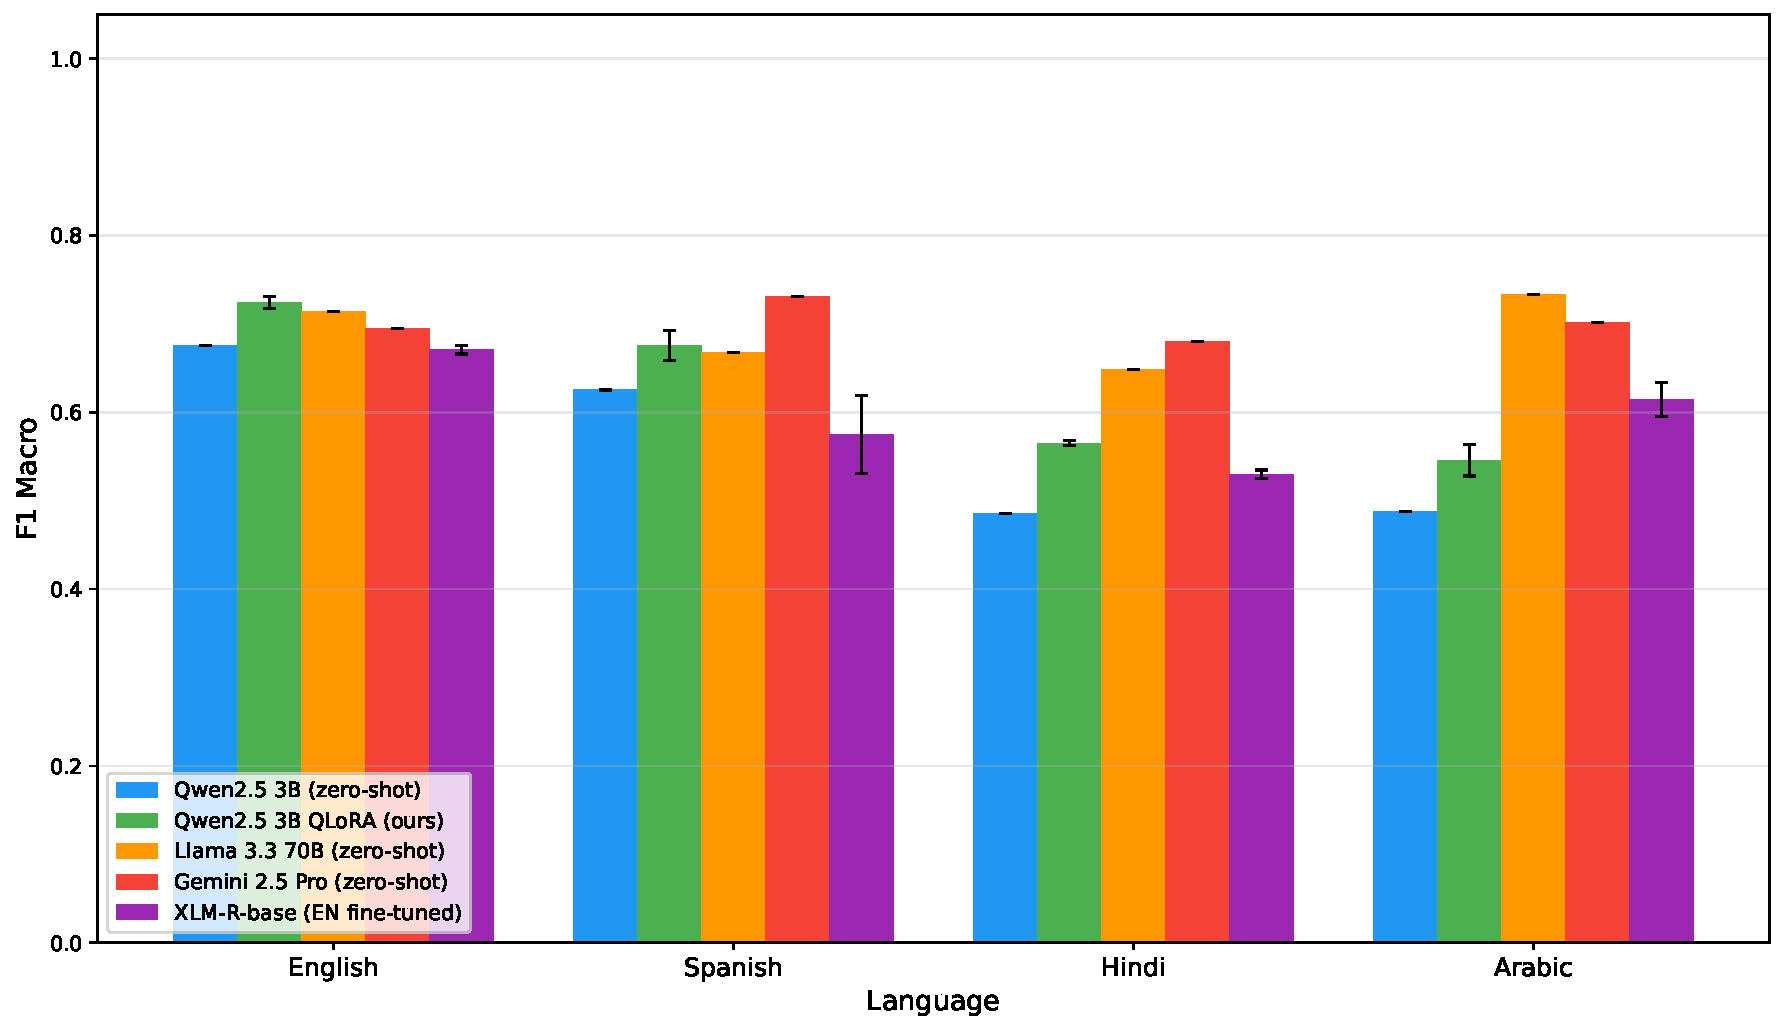
\includegraphics[width=\columnwidth]{figures/f1_grouped_bar.pdf}
\caption{Macro-F1 across the five model configurations and four languages; the
majority baseline (0.1667 everywhere) is omitted for legibility. Error bars are
sample standard deviations over three seeds for QLoRA and \mbox{XLM-R}; the deterministic single-run
configurations have none, and their sampling uncertainty is given as bootstrap
CIs in Table~\ref{tab:main} instead. The two Qwen bars sit level with the frontier
models on English and Spanish and fall well below them on Hindi and Arabic; the
gap that English tuning closes is roughly constant across languages
(\mbox{+0.049} to \mbox{+0.080}), while the gap to the frontier models is not.}
\label{fig:bars}
\end{figure}





\section{Prompt}
\label{app:prompt}
All four generative configurations receive identical text. System message:

\begin{quote}\small\ttfamily
You are a sentiment classifier. Classify the sentiment of the given text as
exactly one of: positive, neutral, or negative. Respond with ONLY the sentiment
label, nothing else.
\end{quote}

\noindent User message:

\begin{quote}\small\ttfamily
Classify the sentiment of the following text as positive, neutral, or negative.

Text: \{text\}
\end{quote}

\section{Training Details}
\label{app:training}

Table~\ref{tab:seeds} gives the selected checkpoint for each seed. QLoRA
validation F1 was not logged during training, so the English column reports
seed-level test macro-F1 from the evaluation run rather than a validation score;
\mbox{XLM-R} reports validation F1 as logged. Checkpoint selection used validation loss
in both cases.

\begin{table}[H]
\centering\small
\setlength{\tabcolsep}{4pt}
\begin{tabular}{@{}llccc@{}}
\toprule
Model & Seed & Epoch & Val.\ loss & F1 \\
\midrule
\multirow{3}{*}{QLoRA}
 & 42  & 3 & 0.1907 & 0.7206$^{\dagger}$ \\
 & 123 & 2 & 0.1955 & 0.7326$^{\dagger}$ \\
 & 456 & 2 & 0.1889 & 0.7200$^{\dagger}$ \\
\midrule
\multirow{3}{*}{XLM-R}
 & 42  & 2 & 0.7470 & 0.644 \\
 & 123 & 3 & 0.7249 & 0.670 \\
 & 456 & 3 & 0.8007 & 0.656 \\
\bottomrule
\end{tabular}
\caption{Selected checkpoints per seed. $^{\dagger}$English \emph{test} macro-F1.}
\label{tab:seeds}
\end{table}



\section{Annotated Error Examples}
\label{app:examples}

Table~\ref{tab:examples} shows representative items from the annotated sample of
\S\ref{sec:qualitative}, with its category label and the Qwen2.5
tokenization of one sentiment- or content-bearing word in context. Arabic is
rendered right to left, so in the split column its first piece is the rightmost.
In the Arabic rows the pieces fall inside the word stem (for example
\emph{al-hud\=u'}, `calmness', is split into the article \emph{al-} and two
pieces of the stem). In the Romanized Hindi rows the pieces are short Latin
strings, several of which coincide with English subwords (\emph{bhot} `very'
becomes \emph{b}\,|\,\emph{hot}). English words are also split (the Qwen2.5
tokenizer gives \emph{calm}\,|\,\emph{ness} for `calmness' in the gloss), so the
table illustrates what the pieces look like rather than how many there are.

\needspace{26\baselineskip}
\section{Error Taxonomy}
\label{app:errors}

Each annotated error received exactly one of six categories: the main reason a
reader of the language would give for the misclassification. Table~\ref{tab:errors}
gives the counts behind \S\ref{sec:qualitative}.

\begin{table}[H]
\centering\small
\setlength{\tabcolsep}{4pt}
\begin{tabular}{@{}lcccc@{}}
\toprule
& & \multicolumn{2}{c}{Hindi} & \\
\cmidrule(lr){3-4}
Category & Spanish & round 1 & all & Arabic \\
\midrule
Tokenization artifact & 1 & 0 & 0  & 4 \\
Ambiguous neutral     & 3 & 2 & 12 & 0 \\
Cultural idiom        & 2 & 2 & 4  & 2 \\
Context dependent     & 1 & 2 & 14 & 2 \\
Code-switching        & 0 & 2 & 14 & 0 \\
Sarcasm / irony       & 1 & 0 & 2  & 0 \\
\midrule
Total                 & 8 & 8 & 46 & 8 \\
\bottomrule
\end{tabular}
\caption{Failure categories over the manually annotated QLoRA misclassifications
that at least two of the three seeds make. For Hindi, ``round 1'' is the initial
sample and ``all'' adds a second, larger random sample; code-switching here
includes non-standard Romanized spellings and abbreviations.}
\label{tab:errors}
\end{table}

\noindent The annotators applied the following criteria.
\textbf{Tokenization artifact:} a nameable sentiment-bearing word is split into pieces
that plausibly lose its meaning (this describes how the error looks; on its cause
see \S\ref{sec:collapse}).
\textbf{Ambiguous neutral:} the tweet is genuinely borderline between neutral and a
polar label, so a reasonable reader could choose either.
\textbf{Cultural idiom:} the sentiment is carried by an idiom, proverb or culturally
specific expression whose literal reading is neutral or misleading.
\textbf{Context dependent:} the sentiment depends on knowing who or what is referred to,
such as a celebrity, a politician, an event or an earlier tweet.
\textbf{Code-switching:} the error is plausibly due to Hindi--English mixing or to
non-standard Romanized spellings and abbreviations (\emph{h} for \emph{hai},
\emph{bhot} for \emph{bahut}).
\textbf{Sarcasm / irony:} the literal sentiment is the opposite of the intended one.

\needspace{38\baselineskip}
\section{Full Per-Class Results}
\label{app:detail}

Table~\ref{tab:perclass} gives per-class F1 for every non-trivial
model--language cell. The body reports only the cells it argues from; this is the
complete grid behind the class-level claims of \S\ref{sec:analysis}, including
the count of 16 of 20 cells in which neutral is the weakest class.

\begin{table}[H]
\centering\scriptsize
\setlength{\tabcolsep}{3pt}
\renewcommand{\arraystretch}{0.85}
\begin{tabular}{@{}llccc@{}}
\toprule
Model & & Neg. & Neu. & Pos. \\
\midrule
\multirow{4}{*}{Qwen2.5 3B}
 & EN & .753 & \textbf{.588} & .685 \\
 & ES & .628 & \textbf{.559} & .688 \\
 & HI & \textbf{.442} & .549 & .465 \\
 & AR & .465 & .565 & \textbf{.435} \\
\midrule
\multirow{4}{*}{Qwen2.5 3B QLoRA}
 & EN & .778 & \textbf{.606} & .789 \\
 & ES & .721 & \textbf{.559} & .748 \\
 & HI & \textbf{.511} & .573 & .612 \\
 & AR & \textbf{.507} & .586 & .544 \\
\midrule
\multirow{4}{*}{XLM-R-base}
 & EN & .739 & \textbf{.532} & .742 \\
 & ES & .680 & \textbf{.361} & .684 \\
 & HI & .531 & \textbf{.493} & .565 \\
 & AR & .656 & \textbf{.551} & .637 \\
\midrule
\multirow{4}{*}{Llama 3.3 70B}
 & EN & .777 & \textbf{.583} & .781 \\
 & ES & .763 & \textbf{.491} & .750 \\
 & HI & .677 & \textbf{.567} & .701 \\
 & AR & .789 & \textbf{.676} & .735 \\
\midrule
\multirow{4}{*}{Gemini 2.5 Pro}
 & EN & .770 & \textbf{.615} & .700 \\
 & ES & .776 & \textbf{.635} & .783 \\
 & HI & .698 & \textbf{.640} & .702 \\
 & AR & .754 & \textbf{.667} & .684 \\
\bottomrule
\end{tabular}
\caption{Per-class F1 for the 20 non-trivial model--language cells; leading
zeros are omitted. The majority baseline is excluded because it scores zero on two
of the three classes by construction. QLoRA and \mbox{XLM-R} are means over seeds
42/123/456; the rest are single runs. \textbf{Bold} marks the weakest class in each
row: it is neutral in 16 of the 20 rows, the exceptions being the four Qwen rows on
Hindi and Arabic (\S\ref{sec:collapse}, \S\ref{sec:hindi}). Macro-F1 for every cell is in
Table~\ref{tab:main}.}
\label{tab:perclass}
\end{table}
\renewcommand{\arraystretch}{1}

\section{Label Probabilities and Target-Language Instructions}
\label{app:c1c2}

We re-ran the base model and the three tuned checkpoints on all four test sets with
the original loader, prompt, batching and greedy decoding, and recorded the
log-probability of each label word at the first output step, summed over its
lower-case, capitalised and space-prefixed tokens. For every item the most probable
first token was a label word.
Per-class AUC is computed one-vs-rest from the softmax over the three label
probabilities. The balanced decision rule adds one offset per class, found
iteratively, until each class receives a third of the predictions; it uses the
known class balance of the test set and no item labels. For the target-language
condition the system and user messages of Appendix~\ref{app:prompt} were translated
into Spanish, Romanized Hindi and Modern Standard Arabic, with the Romanized Hindi
version checked by the author as a native speaker, and the label words kept in English so that outputs are scored
exactly as before; the Romanized Hindi user message, for example, reads
\textit{Neeche diye gaye text ka sentiment positive, neutral, ya negative mein
batao.} The exact prompts are in the released notebook.

\begin{table}[H]
\centering\small
\setlength{\tabcolsep}{2.5pt}
\begin{tabular}{@{}lccccccc@{}}
\toprule
& \multicolumn{2}{c}{EN instr.} & \multicolumn{3}{c}{AUC} & Bal. & \multicolumn{1}{c}{Target} \\
\cmidrule(lr){2-3}\cmidrule(lr){4-6}
Lang. & F1 & neu.\% & neg & neu & pos & F1 & F1 / neu.\% \\
\midrule
EN & .724 & 32.0 & .929 & .797 & .948 & .738 & --- \\
ES & .676 & 29.1 & .899 & .774 & .901 & .687 & .659 / 20.7 \\
HI & .565 & 55.2 & .797 & .718 & .810 & .599 & .577 / 34.0 \\
AR & .546 & 69.3 & .885 & .778 & .871 & .669 & .665 / 26.1 \\
\bottomrule
\end{tabular}
\caption{QLoRA, mean over three seeds. ``EN instr.'': the main results
(Tables~\ref{tab:main} and \ref{tab:neutral}). ``Bal.'': macro-F1 under the
balanced decision rule. ``Target'': macro-F1 and neutral share with the instruction
in the target language. Seed standard deviations are at most 0.016 for AUC and
0.012 for the balanced and target-language F1. The untuned base model behaves similarly: on Arabic,
the balanced rule gives 0.650 and the Arabic instruction 0.671 (from 0.488); on
Hindi, 0.572 and 0.539 (from 0.485).}
\label{tab:c1c2}
\end{table}

\needspace{12\baselineskip}
\section{Fragmentation Measures}
\label{app:parity}

\begin{table}[H]
\centering\small
\setlength{\tabcolsep}{3pt}
\begin{tabular}{@{}lccccc@{}}
\toprule
& Tok./ & \multicolumn{2}{c}{Parity (MT, full split)} & \multicolumn{2}{c}{Parity, $n{=}10$} \\
\cmidrule(lr){3-4}\cmidrule(lr){5-6}
Lang. & word & pooled [95\% CI] & words & human & MT \\
\midrule
English & 1.633 & 1 (ref.) & 1 & --- & --- \\
Spanish & 1.582 & 1.22 [1.21, 1.24] & 0.92 & 1.11 & 1.21 \\
Hindi   & 1.703 & 1.26 [1.24, 1.28] & 0.98 & 1.33 & 1.36 \\
Arabic  & 2.592 & 1.41 [1.39, 1.43] & 0.71 & 1.24 & 1.30 \\
\bottomrule
\end{tabular}
\caption{Fragmentation under the Qwen2.5 tokenizer: tokens per word, parity with a
1{,}000-resample bootstrap CI, word-count ratio, and parity against human and
machine translations of the annotated items.}
\label{tab:parity}
\end{table}


Table~\ref{tab:parity} compares the two fragmentation measures. Tokens per word is
the more common measure, computed here on the raw test text; parity is computed on cleaned text against machine translations
(\S\ref{sec:setup}). The word ratio shows why tokens per word overstates Arabic:
Arabic tweets have far fewer whitespace-separated words than their English
translations. The validation columns use the 10 items per language of the first
annotation round, which have human translations (\S\ref{sec:qualitative}). Four Hindi items contain nothing
but hashtags, mentions or links, are empty after cleaning, and are excluded
(Hindi $n{=}866$). The human-translated sample is too small to rank languages: it
places Hindi above Arabic, where the full machine-translated set does not.

\section{Confusion Matrices}
\label{app:confusion}


\noindent Figure~\ref{fig:confusion} is the raw evidence behind the prediction
rates in Tables~\ref{tab:neutral} and \ref{tab:collapse}; three of its cells carry the
argument of \S\ref{sec:analysis}. In the QLoRA row of the Arabic column, 59.5\% of
true negatives and 58.2\% of true positives are routed to neutral while 90.2\% of
true neutrals are retained~--- a near-vertical band rather than a diagonal. The
Hindi column of that row shows the same shape more mildly, with 49.7\% of negatives
and 39.9\% of positives lost to neutral (\S\ref{sec:hindi}). The \mbox{XLM-R} row of the
Spanish column inverts it: only 26.8\% of true neutrals are recovered, with 43.2\%
pushed to positive and 30.0\% to negative, so the neutral \emph{row} empties into the
polar columns instead. Llama 3.3 70B on Arabic is diagonal-dominant throughout
(76.9\%, 74.1\%, 68.3\%)~--- what the absence of a collapse looks like at this scale.



\begin{figure}[H]
\centering
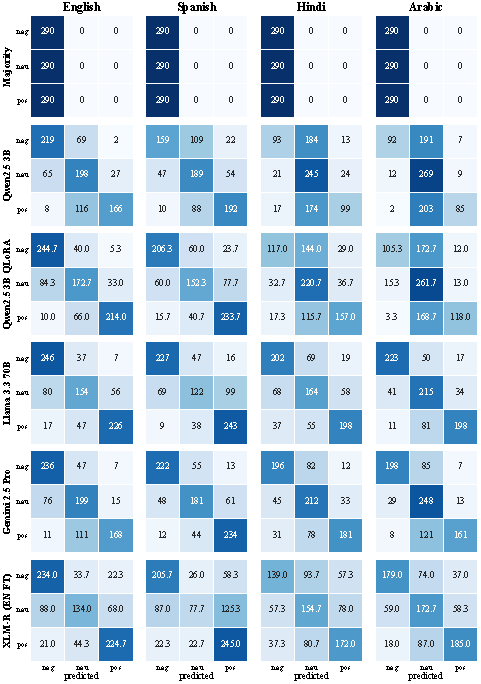
\includegraphics[width=\columnwidth]{figures/confusion_matrices_grid.pdf}
\caption{Confusion matrices for all 24 model--language combinations, 870 test
examples each; rows are configurations, columns are languages. Cells are counts,
and for the two seed-dependent models (QLoRA, \mbox{XLM-R}) they are means over seeds
42/123/456~--- hence the decimals~--- so that every rate quoted in
Tables~\ref{tab:neutral} and \ref{tab:collapse} can be read directly off this
figure.}
\label{fig:confusion}
\end{figure}

\end{document}
